Aplikacja konsolowa powstała w celu przetwarzania czasochłonnych zadań w tle, tak by użytkownik aplikacji webowej nie doświadczał długich czasów ładowania oraz ewentualnych błędów podczas przerwania sesji. Aplikacja konsolowa uruchamiana jest co 5 minut i przetwarza zadania trzech typów w kolejności widocznej na rysunku \ref{fig:worker_proces}. Poszczególne procesy zostały szerzej opisane w kolejnych podrozdziałach.
\begin{figure}[H]
	\centering
	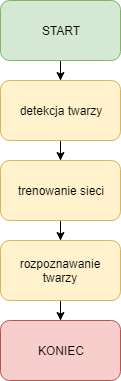
\includegraphics[scale=0.6]{worker_proces.png}
	\caption{Proces działania aplikacji konsolowej}
	\label{fig:worker_proces}
\end{figure}

\section{Technologie}
Aplikacja konsolowa powstała w języku programowania Python w wersji trzeciej. W początkowej fazie projektu za wyborem tego języka przemawiała wieloplatformowość, możliwości wprowadzania szybkich zmian w kodzie i brak potrzeby go kompilowania. C\#, który został wybrany do stworzenia aplikacji webowej okazał się nie przystosowany do modyfikowania kodu na platformie Raspberry Pi z powodu braku dostępnego .NET Core SDK na procesory ARM, a uruchomienie programu wymagało znacznie większej ilości zasobów obliczeniowych niż Python. Ostatecznie aplikacja konsolowa została przeniesiona na zewnętrzny serwer. Popularność Pythona pozwoliła na
integrację z wybranymi usługami dzięki dostępności SDK (Software Developmnet Kit).

\section{Proces wykrywania twarzy}
Uogólniony proces detekcji twarzy na obrazie został przedstawiony na grafie \ref{fig:wykrywanie_proces}.
Proces przetwarzania zadań detekcji rozpoczyna się od pobrania z bazy wszystkich żądań o statusie 'New'. Następnie każde zadanie przetwarzane jest osobno. Dla aktualnie procesowanego zadania pobierany jest obraz wejściowy z usługi Dropbox i zapisywany w lokalnym folderze. Następnym krokiem jest wywołanie procesu odpowiedzialnego za preprocessing zdjęcia i pozyskanie oczekiwanych wyników detekcji. Krok ten został szerzej opisany w podrozdziałach \ref{detekcja_haar}, \ref{detekcja_dnn} i \ref{detekcja_azure}. Po uzyskaniu wyników każdą dostępną w programie metodą, utworzony zostaje obraz wyjściowy dla każdej metody (haar, azure, ..), który program uploaduje do odpowiedniego folderu w usłudze Dropbox. Po poprawnym wgraniu plików wynikowych następuje zapisanie informacji o rezultatach w bazie danych. Po wykonaniu zadania bez żadnych błędów request zostaje oznaczony jako zakończony. W innym przypadku status zostaje zmieniony na 'Error'. Proces powtarzany jest dla każdego wpisu pozyskanego z bazy.
\begin{figure}[H]
	\centering
	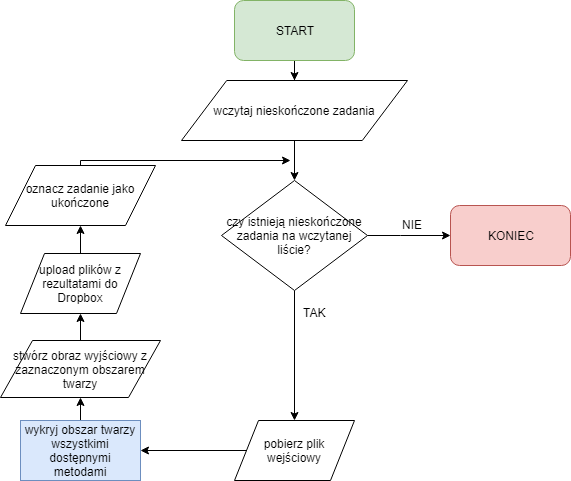
\includegraphics[scale=0.6]{wykrywanie_twarzy.png}
	\caption{Proces wykrywania twarzy zaimplementowany w aplikacji konsolowej}
	\label{fig:wykrywanie_proces}
\end{figure}

\subsection{OpenCv Haar} \label{detekcja_haar}
Pierwszą z metod detekcji twarzy, która została zintegrowana z programem jest detekcja metodą Haar'a. Algorytm został opisany w rozdziale \ref{haar}. Przed uruchomieniem detekcji obraz wejściowy należy odpowiednio przygotować. W tym celu wcześniej pobrany obraz zostaje wczytany do programu i przekonwertowany do odcieni szarości. Tak przygotowany obraz można poddać detekcji. Detektor zwraca współrzędne obszarów zawierających w sobie twarz. Tak uzyskane dane należy przekonwertować do formatu, który został przyjęty jako wspólny dla wszystkich metod.
\begin{figure}[H]
	\centering
	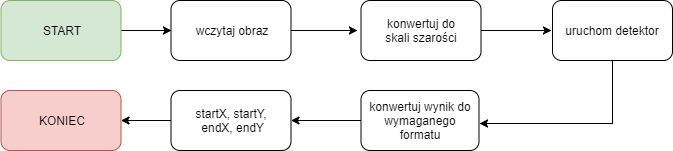
\includegraphics[scale=0.6]{detekcja_haar.png}
	\caption{Wykrywanie twarzy metodą Haar zaimplementowane w aplikacji konsolowej}
	\label{fig:wykrywanie_haar}
\end{figure}

\subsection{OpenCv DNN (Deep Neural Network)} \label{detekcja_dnn}
Proces detekcji z wykorzystaniem głęboko uczonej sieci neuronowej nie wymaga formatowania obrazu do skali szarości, ale za to obraz musi zostać przeskalowany do odpowiedniego, wcześniej przyjętego rozmiaru. Dodatkową zaletą tej metody jest format odpowiedzi detektora, który oprócz obszaru zawierającego twarz zwraca również 'pewność' z jaką twarz została wykryta, co pozwala na odfiltrowanie wyników poniżej pewnego poziomu.
\begin{figure}[H]
	\centering
	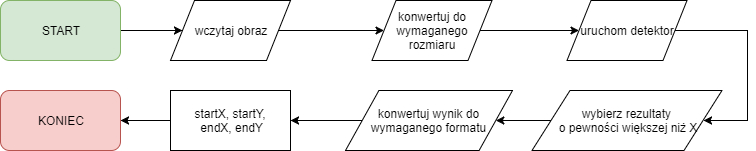
\includegraphics[scale=0.6]{detekcja_dnn.png}
	\caption{Wykrywanie twarzy metodą DNN (Deep Neural Network) zaimplementowane w aplikacji konsolowej}
	\label{fig:wykrywanie_dnn}
\end{figure}

\subsection{Azure Cognitive Services} \label{detekcja_azure}
Podczas detekcji twarzy przy pomocy Azure Cognitive Services wszystkie operacje przetwarzania obrazu wykonywane są w chmurze co pozwala odciążyć środowisko rozruchowe. Proces wykrycia twarzy ogranicza się do przesłania wybranego obrazu do ACS Api (Application programming interface). Lokalnie nie jest wykonywany żaden preprocessing. W odpowiedzi klient Api uzyskuje wiadomość JSON zawierającą skonfigurowane podczas zapytania parametry. JSON zostaje zparsowany do postaci obiektu ze wszystkimi informacjami. Wartości zostają przekonwertowane do formatu [startX, startY, endX, endY].
\begin{figure}[H]
	\centering
	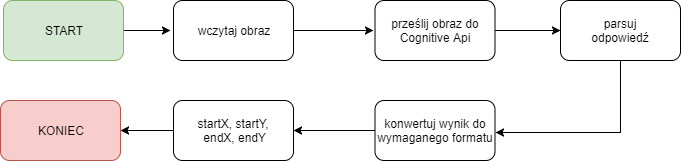
\includegraphics[scale=0.6]{detekcja_azure.png}
	\caption{Wykrywanie twarzy używając Azure Cognitive Services zaimplementowane w aplikacji konsolowej}
	\label{fig:wykrywanie_azure}
\end{figure}

\section{Proces trenowania modelu dla wybranych algorytmów}
Uproszczony proces trenowania grupy identyfikatorów twarzy przedstawiono na grafie \ref{fig:trenowanie_proces}. Po jego zakończeniu użytkownik otrzymuję grupę z wytrenowanymi modelami gotową do wykorzystania w zakładce 'Recognitions'.
Proces zaczyna się od sprawdzenia jakie dane uczące (profile utworzone w zakładce 'Profiles' aplikacji webowej) są dostępne lokalnie. Repozytorium zostaje porównane z danymi dostępny w bazie, a następnie zaktualizowane o brakujące profile.
\begin{figure}[H]
	\centering
	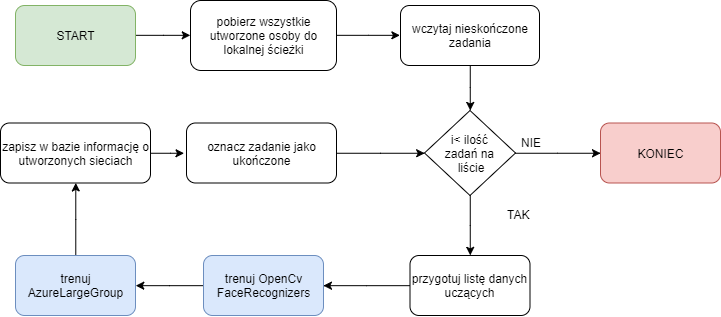
\includegraphics[scale=0.6]{proces_nauczania.png}
	\caption{Proces trenowania sieci zaimplementowany w aplikacji konsolowej}
	\label{fig:trenowanie_proces}
\end{figure}
W kolejnym kroku następuje pobranie z bazy wszystkich requestów, które nie zostały jeszcze zakończone. Następnie dla każdego zgłoszenia z listy wykonywany jest proces przygotowania listy danych uczących, które wybrano podczas tworzenia zadania w aplikacji webowej. Kolejne dwa kroki są specyficzne dla danego algorytmu dlatego 'trenuj OpenCv FaceRecognizers' opisano w rozdziale \ref{trenowanie_open_cv}, a 'trenuj AzureLargeGroup' w \ref{trenowanie_azure}. Po zakończeniu trenowania zintegrowanych algorytmów następuje proces zapisu danych o utworzonych modelach sieci w bazie danych.
W przypadku braku komplikacji, request zostaje oznaczony jako zakończony. Proces zostaje powtórzony dla każdego zadania wczytanego do listy na początku grafu \ref{fig:trenowanie_proces}.

\subsection{Trenowanie identyfikatorów OpenCv} \label{trenowanie_open_cv}
Ogólny schemat procesu trenowania identyfikatorów twarzy OpenCv (Eigenfaces, Fisherfaces, LBPH) został przedstawiony na rysunku \ref{fig:trenowanie_open_cv}. Zalecany proces trenowania udostępniony w dokumentacji \cite{opencv_doc} został poddany zmianom wymaganym przez aplikację konsolową i zaimplementowany.
\begin{figure}[H]
	\centering
	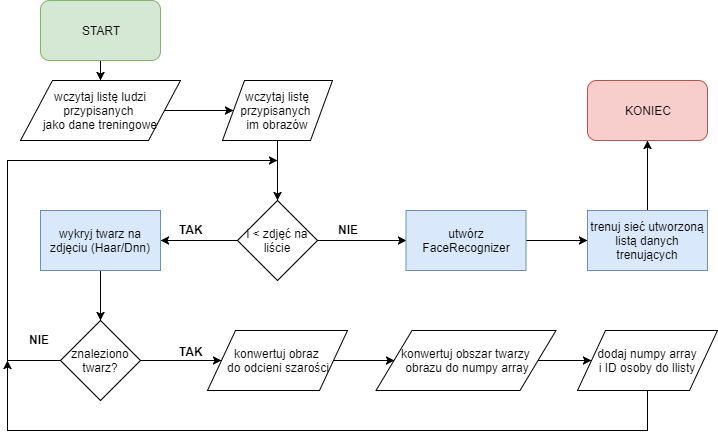
\includegraphics[scale=0.6]{trenowanie_open_cv.png}
	\caption{Trenowanie algorytmów z biblioteki OpenCv zaimplementowane w aplikacji konsolowej}
	\label{fig:trenowanie_open_cv}
\end{figure}
Proces rozpoczyna się od stworzenia listy zawierającej wszystkie przypisane do sieci profile oraz załączone do nich obrazy. Następnie dla każdego zdjęcia z listy zostaje wykonany preprocessing. Pierwszym krokiem jest próba wykrycia twarzy na obrazie. W przypadku nie znalezienia twarzy, obraz zostaje zignorowany i program przechodzi do przetwarzania kolejnego obrazu. Jeśli na zdjęciu zostanie zlokalizowana twarz, to obszar ją zawierający zostaje przeskalowany do odcieni szarości, a następnie przekonwertowany do postaci numpy array. Wektor zawierający informację o twarzy zostaje dodany do listy uczącej wraz z ID profilu, do którego należy zdjęcie. 

Po przetworzeniu wszystkich obrazów na liście, następuje utworzenie FaceRecognizera dla wszystkich 3 metod dostępnych w bibliotece OpenCv. W kolejnym kroku następuje wytrenowanie modeli danymi z przygotowanej w poprzednich krokach listy uczącej. Trenowanie wykonywane jest w kolejności LBPH, Eigen, a na końcu Fisher. Ostatnim krokiem jest utworzenie plików modelu dla każdego z algorytmów, które następnie zostają wgrane do folderu w usłudze Dropbox.


\subsection{Trenowanie identyfikatora Azure} \label{trenowanie_azure}
Proces rozpoczyna się od wczytania wszystkich profili oraz ich zdjęć, które zostały przypisane do zadania trenowania sieci. Na diagramie \ref{fig:trenowanie_azure} niebieskim kolorem oznaczono zapytania do Azure Cognitive Services API(Application Programming Interface).
\begin{figure}[H]
	\centering
	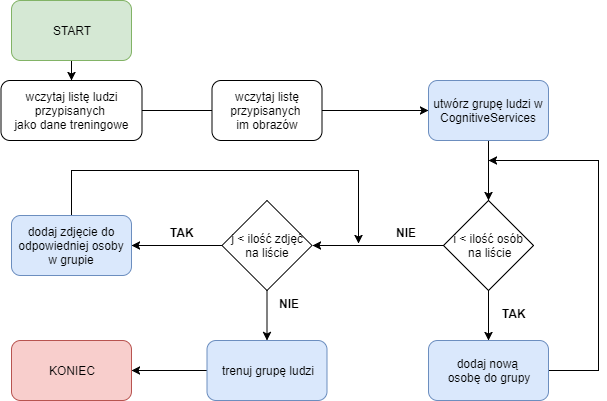
\includegraphics[scale=0.55]{trenowanie_azure.png}
	\caption{Trenowanie usługi Azure Cognitive Services zaimplementowane w aplikacji konsolowej}
	\label{fig:trenowanie_azure}
\end{figure}
Zgodnie z dokumentacją \cite{acs_doc} pierwszym i najważniejszym krokiem jest utworzenie AzureLargeGroup, do której w kolejnym kroku zostaną dodane id/nazwy wszystkich profili znajdujących się na wczytanej liście.  Następnie każdy obraz z listy zostaje przypisany odpowiedniej osobie w AzureLargeGroup. W tym rozwiązaniu klient nie musi martwić się detekcją twarzy na obrazie, bo jest ona wykonywana przez usługę Azure po przesłaniu obrazu. W przypadku problemów z detekcją twarzy Api Azure'a zwróci błąd, który jest logowany w aplikacji. W takiej sytuacji obraz zostanie potraktowany jako zignorowany i proces wgrywania kolejnych zdjęć będzie kontynuowany. Po dodaniu wszystkich zdjęć, program wywołuje funkcję trenowania. Danymi uczącymi są osoby, które utworzono w AzureLargeGroup. Nawet dla 2 tysięcy zdjęć proces trenowania jest wyjątkowo krótki i kończy się po około jednej sekundzie.

Ze względu na setki zapytań HTTP, które muszą zostać wykonane do zewnętrznego serwisu Azure proces przygotowania danych przed trenowaniem może wydłużyć się nawet do kilku minut w przypadku wybrania szerokiego zakresu danych uczących.

\section{Proces rozpoznawania twarzy}\label{s:proces_rozpoznawania}
Ogólny proces rozpoznawania twarzy przedstawiony na rysunku \ref{fig:rozpoznawanie_proces} jest zbliżony do wcześniej opisywanych procesów detekcji i trenowania. 

Proces rozpoczyna się od pobrania wszystkich wytrenowanych modeli, których aktualnie nie ma w lokalnym katalogu. W kolejnym etapie wczytane zostają wszystkie nowe zadania rozpoznania twarzy. Dla każdego z requestów na liście wykonywane są te same czynności, a pierwszą z nich jest pobranie pliku wejściowego z usługi Dropbox. Następnie twarz zostaje rozpoznana za pomocą każdego dostępnego algorytmu identyfikacji z biblioteki OpenCv oraz AzureLargeGroup. 

Identyfikację przy użyciu OpenCv opisano w rozdziale \ref{{s:identyfikacja_opencv}}, a wykorzystując AzureLargeGroup. Po ukończeniu identyfikacji tożsamości zadanie zmienia status na ukończone. Proces powtarza się w pętli aż do ukończenia wszystkich zadań z początkowo wczytanej listy.
\begin{figure}[H]
	\centering
	\includegraphics[scale=0.6]{rozpoznawanie_twarzy.png}
	\caption{Proces identyfikacji tożsamości zaimplementowany w aplikacji konsolowej}
	\label{fig:rozpoznawanie_proces}
\end{figure}

\subsection{Identyfikacja tożsamości metodami dostępnymi w OpenCv}\label{s:identyfikacja_opencv}
Proces rozpoznania twarzy metodami dostępnymi w bibliotece OpenCv został skonstruowany na podstawie przykładu przedstawionego w dokumentacji \cite{opencv_doc}. Zmodyfikowany na potrzeby programu przebieg procesu ukazano na rysunku \ref{fig:rozpoznawanie_open_cv}.
\begin{figure}[H]
	\centering
	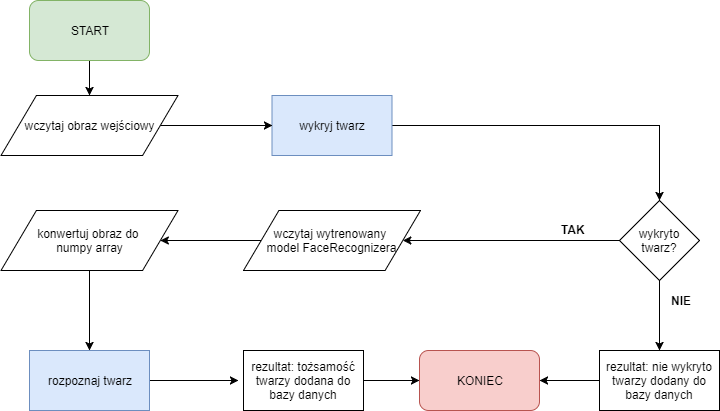
\includegraphics[scale=0.6]{rozpoznawanie_open_cv.png}
	\caption{Proces identyfikacji osoby wykorzystując identyfikatory OpenCv zaimplementowany w aplikacji konsolowej}
	\label{fig:rozpoznawanie_open_cv}
\end{figure}
Obraz zostaje wczytany do programu, a następnie zostaje podjęta próba detekcji twarzy metodą Haara lub Dnn (Deep neural network). W przypadku nie wykrycia żadnej twarzy do zadania zostaje dodany pusty rezultat z komentarzem informującej o braku twarzy na przekazanym obrazie. 
Jeśli na zdjęciu zostanie wykryta twarz to proces przechodzi do kolejnego kroku, którym jest utworzenie FaceRecognizera dla każdego dostępnego modelu przypisanego do zadania. Przed identyfikacją wycinek obrazu zawierający twarz zostaje przekonwertowany do numpy array, który jest formatem wymaganym przez FaceRecognizer. W rezultacie uzyskana zostaje tożsamość osoby ze zdjęcia prezentowana w postaci numeru Id z bazy oraz wartość wektora oddalenia od najbliższego obiektu w modelu. Wartość 0,0 oznacza idealne dopasowanie. Im większa wartość tym mniejsza pewność identyfikacji. 


\subsection{Identyfikacja tożsamości przy użyciu Azure Cognitive Services}\label{s:identyfikacja_azure}
Proces rozpoznawania twarzy przy pomocy Azure Cognitive Services jest mniej obciążający dla platformy, na której uruchomiono program. Największą wadą rozwiązania jest uzależnienie szybkości identyfikacji od jakości połączenia z serwisem Azure oraz rozmiaru zdjęcia, a raczej prędkości przesyłania go protokołem HTTP.

Kroki procesu identyfikacji zaimplementowano zgodnie z przykładem przedstawionym w dokumentacji \cite{acs_doc}. Pierwszym z nich jest wczytanie ścieżki do pliku, który następnie zostaje przesłany do usługi Azure w celu detekcji twarzy. Proces detekcji opisano w rozdziale \ref{detekcja_azure}. Zapytanie zostaje zmodyfikowane i zamiast obszaru wykrycia zwrócony zostaje numer identyfikacyjny przypisany do wykrytej twarzy przechowywanej w chmurze.
\begin{figure}[H]
	\centering
	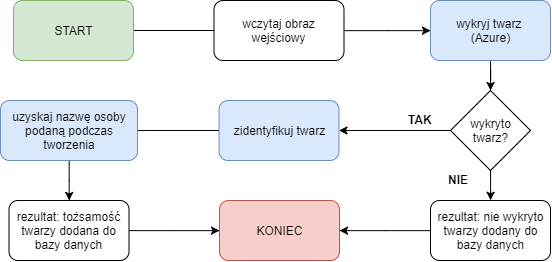
\includegraphics[scale=0.6]{rozpoznawanie_azure.png}
	\caption{Proces identyfikacji osoby wykorzystując Azure Cognitive Servces zaimplementowany w aplikacji konsolowej}
	\label{fig:rozpoznawanie_azure}
\end{figure}
W przypadku nie wykrycia twarzy informacja o problemie z detekcją zostaje zapisana w bazie danych i proces się kończy. W sytuacji gdy twarz została wykryta pomyślnie to wykonane zostaje zapytanie do AzureLargeGroup o numerze przypisanym do zadania identyfikacji. Jedynym parametrem przekazanym podczas zapytania jest unikalny numer twarzy nadany w poprzednim kroku. Odpowiedź systemu ma postać wiadomości w formacie JSON zawierającej tożsamość w postaci numeru guid nadanego osobie przez Azure oraz pewność identyfikacji w postaci wartości z zakresu 0 do 1. W celu poznania numeru Id istniejącego w bazie danych aplikacji wykonywane jest kolejne zapytanie do chmury, w wyniku którego uzyskuje się numer Id użyty podczas dodawania osoby do AzureLargeGroup. W ostatnim kroku uzyskany wynik zostaje zapisany do bazy danych.


